\section{Metodología}
\subsection{Propuesta de solución}
\label{propuesta_solucion}
La solución propuesta consiste en desarrollar un sistema web desde cero siguiendo la arquitectura MVC con el framework ASP.NET Core (.NET 10), con persistencia de datos en SQL Server y almacenamiento en la nube por medio de AWS S3. El sistema consta de dos módulos, el módulo de conversion y carga de archivos, que permite subir documentos en distintos formatos para su conversión a PDF, asi como imágenes y enlaces. Y el módulo de gestión documental, que permite ver todos los archivos almacenados en el sistema y generar codigos QR para cada uno de ellos, asi como la visualización, la eliminación o la descarga de los archivos, todo desde una misma plataforma.

El proceso de autenticación se integra con el mecanismo existente en la institucion, ya que esta plataforma solo sera accedida como una extensión de sistemas que ya tienen su proceso de autenticación.

\subsubsection{Beneficios del sistema propuesto}
Al implementar esta propuesta la gestión documental del PJETAM mejoraria en la accesibilidad de los documentos, ya que sería más fácil el poder acceder a los documentos mediante su código QR ya sea digital o impreso, el sistema también hace mas fácil el proceso de almacenar los documentos en un mismo sitio, y hace los procedimientos más fáciles al hacerlo en la misma plataforma, quitando la necesidad de usar herramientas externas.
%
\subsection{Análisis del sistema}

\subsubsection{Diagramas de flujo del sistema}
\paragraph{Flujo del módulo de conversión y carga de archivos}
El diagrama de la Figura \ref{fig:diagrama_1} muestra el flujo del sistema al convertir y almacenar un archivo, ya sea un documento o un enlace, ilustra el flujo desde que el usuario ingresa hasta que el archivo queda registrado en la base de datos y ya visible en el módulo de gestión.
\begin{figure}[!tbh]
    \centering
    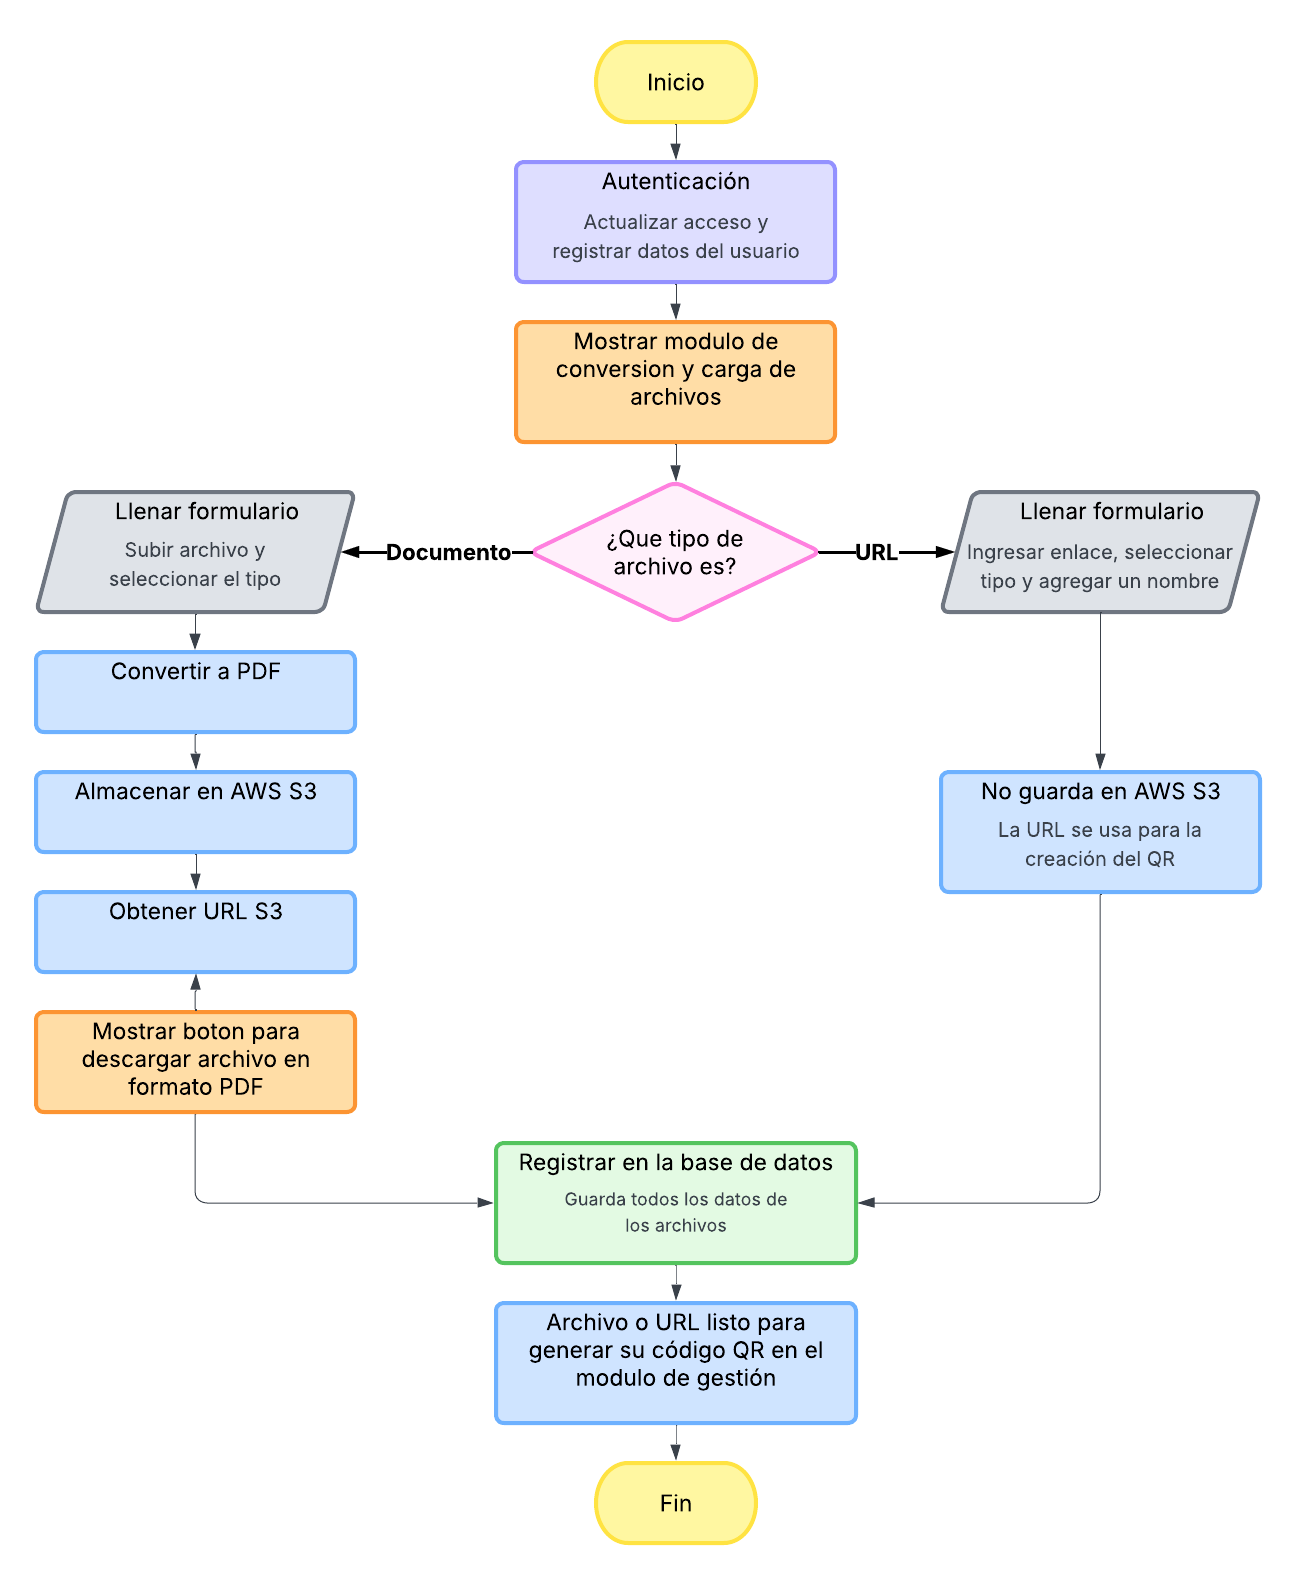
\includegraphics[width=0.9\linewidth]{img/diagrama_conversion.png}
    \caption{Diagrama de flujo: Módulo de conversión y carga de archivos. Fuente: elaboración propia}
    \label{fig:diagrama_1}
\end{figure}

\paragraph{Flujo del módulo de gestión documental}
La Figura \ref{fig:diagrama_2} muestra el flujo de este módulo, en el cual se pueden gestionar todos los archivos almacenados en el sistema, en la lista solo se muestran los archivos que no han sido eliminados y como se ve en la figura, por cada archivo se pueden hacer cuatro acciones, entre ellas la creación de códigos QR para cada archivo, los cuales tambien se guardan en la base de datos con las relaciones de su archivo.
\begin{figure}[!tbh]
    \centering
    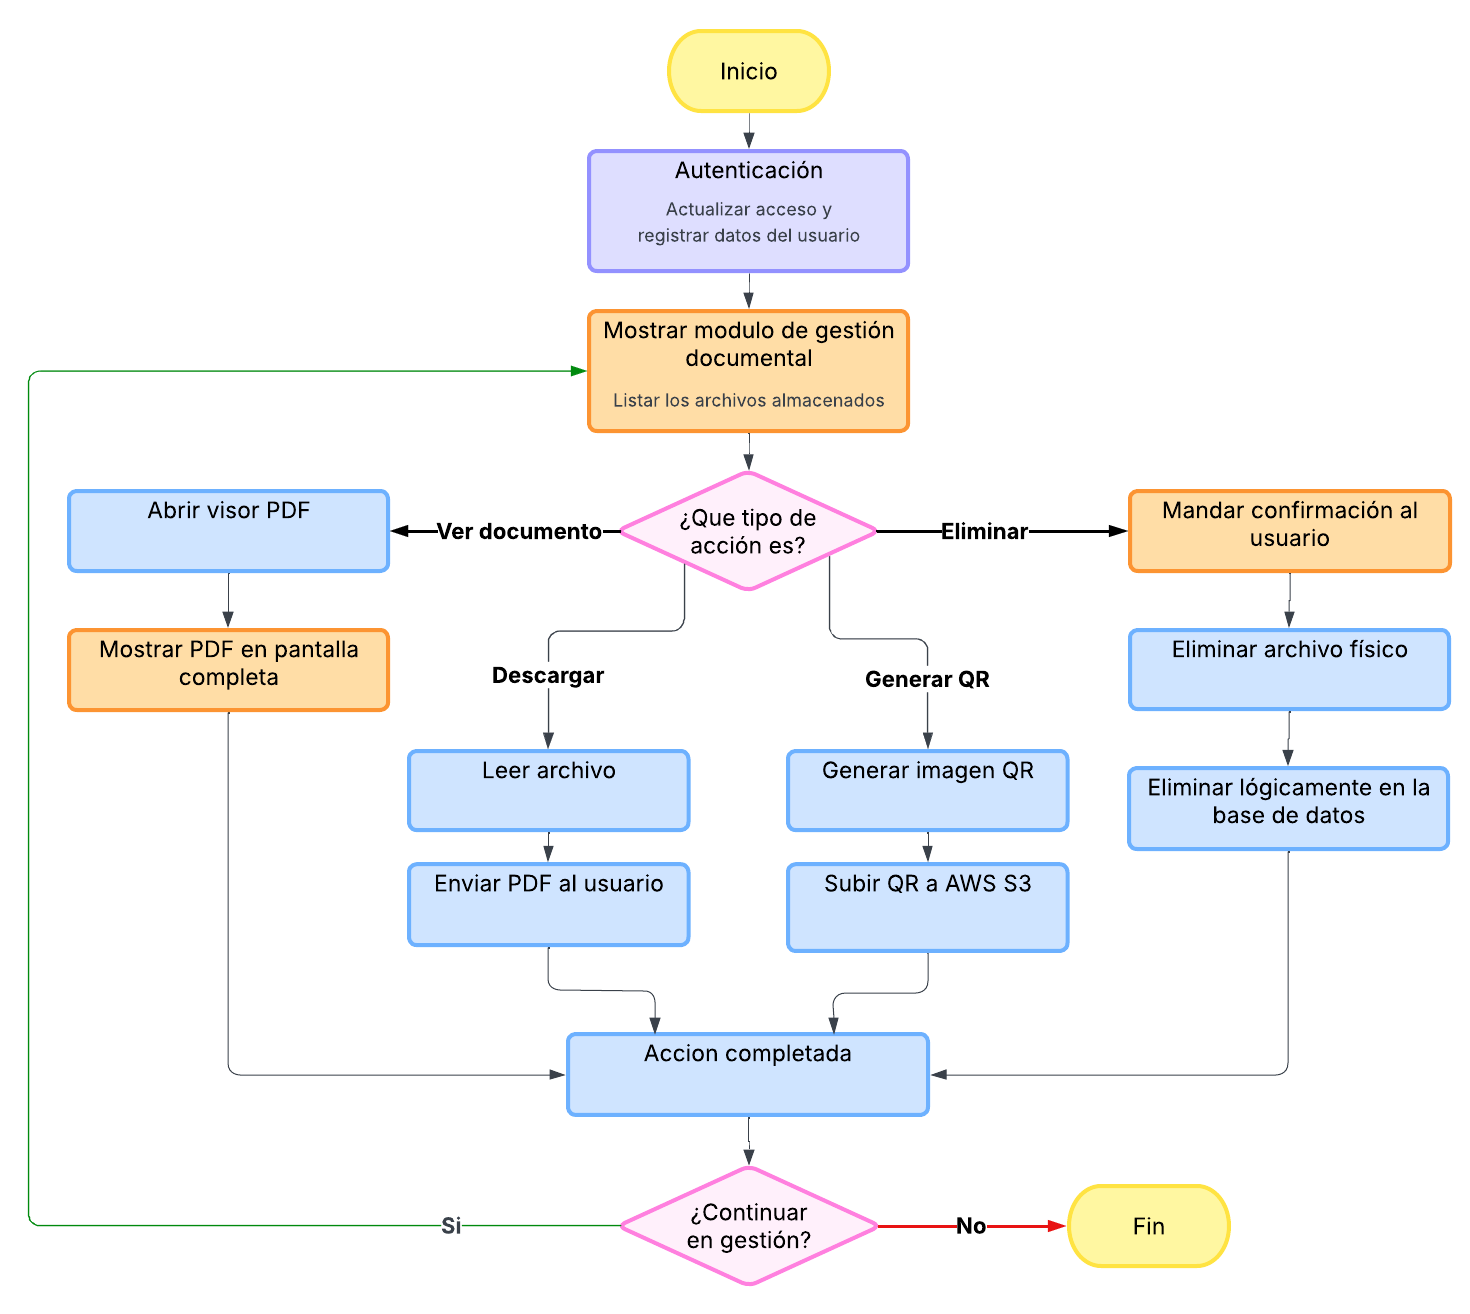
\includegraphics[width=0.9\linewidth]{img/diagrama_gestion.png}
    \caption{Diagrama de flujo: Módulo de gestión documental. Fuente: elaboración propia}
    \label{fig:diagrama_2}
\end{figure}

\subsubsection{Diagrama de caso de uso}

\subsubsection{Diagramas de actividades}


\subsection{Diseño del sistema}
\label{diseño_sistema}

\subsubsection{Diagrama de Entidad-Relación de la Base de Datos}
En la Figura \ref{fig:modelo-er}
\begin{figure}[!tbh]
    \centering
    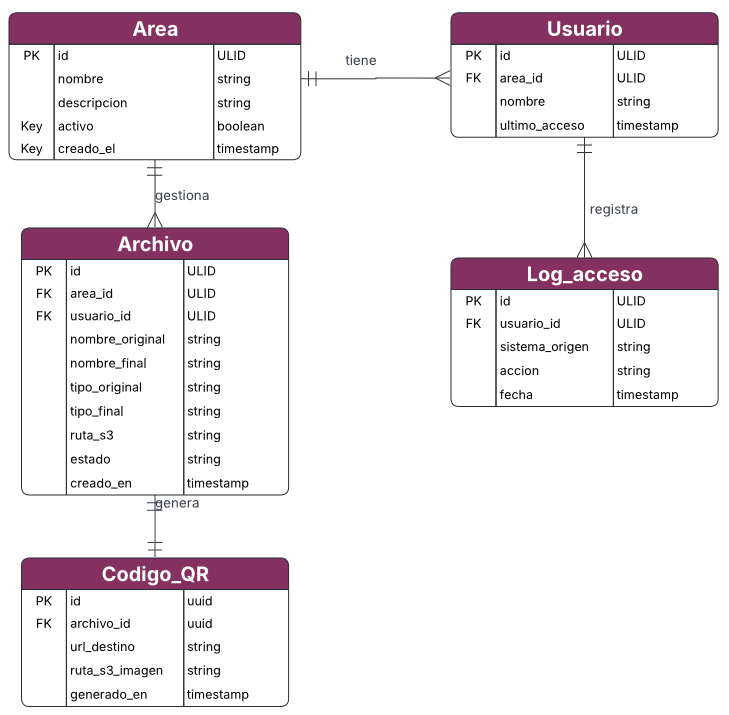
\includegraphics[width=0.7\linewidth]{img/modelo ER.jpeg}
    \caption{Modelo Entidad-Relación del sistema. Fuente: elaboración propia}
    \label{fig:modelo-er}
\end{figure}

\subsubsection{Diagramas de secuencia}

\subsubsection{Diseño de interfaz}
Para la propuesta del sistema se realizaron dos vistas principales para dividir los módulos más importantes del sistema

\paragraph{Modulo de conversion y carga de archivos}
En la Figura \ref{fig:mockup-1}
\begin{figure}[!tbh]
    \centering
    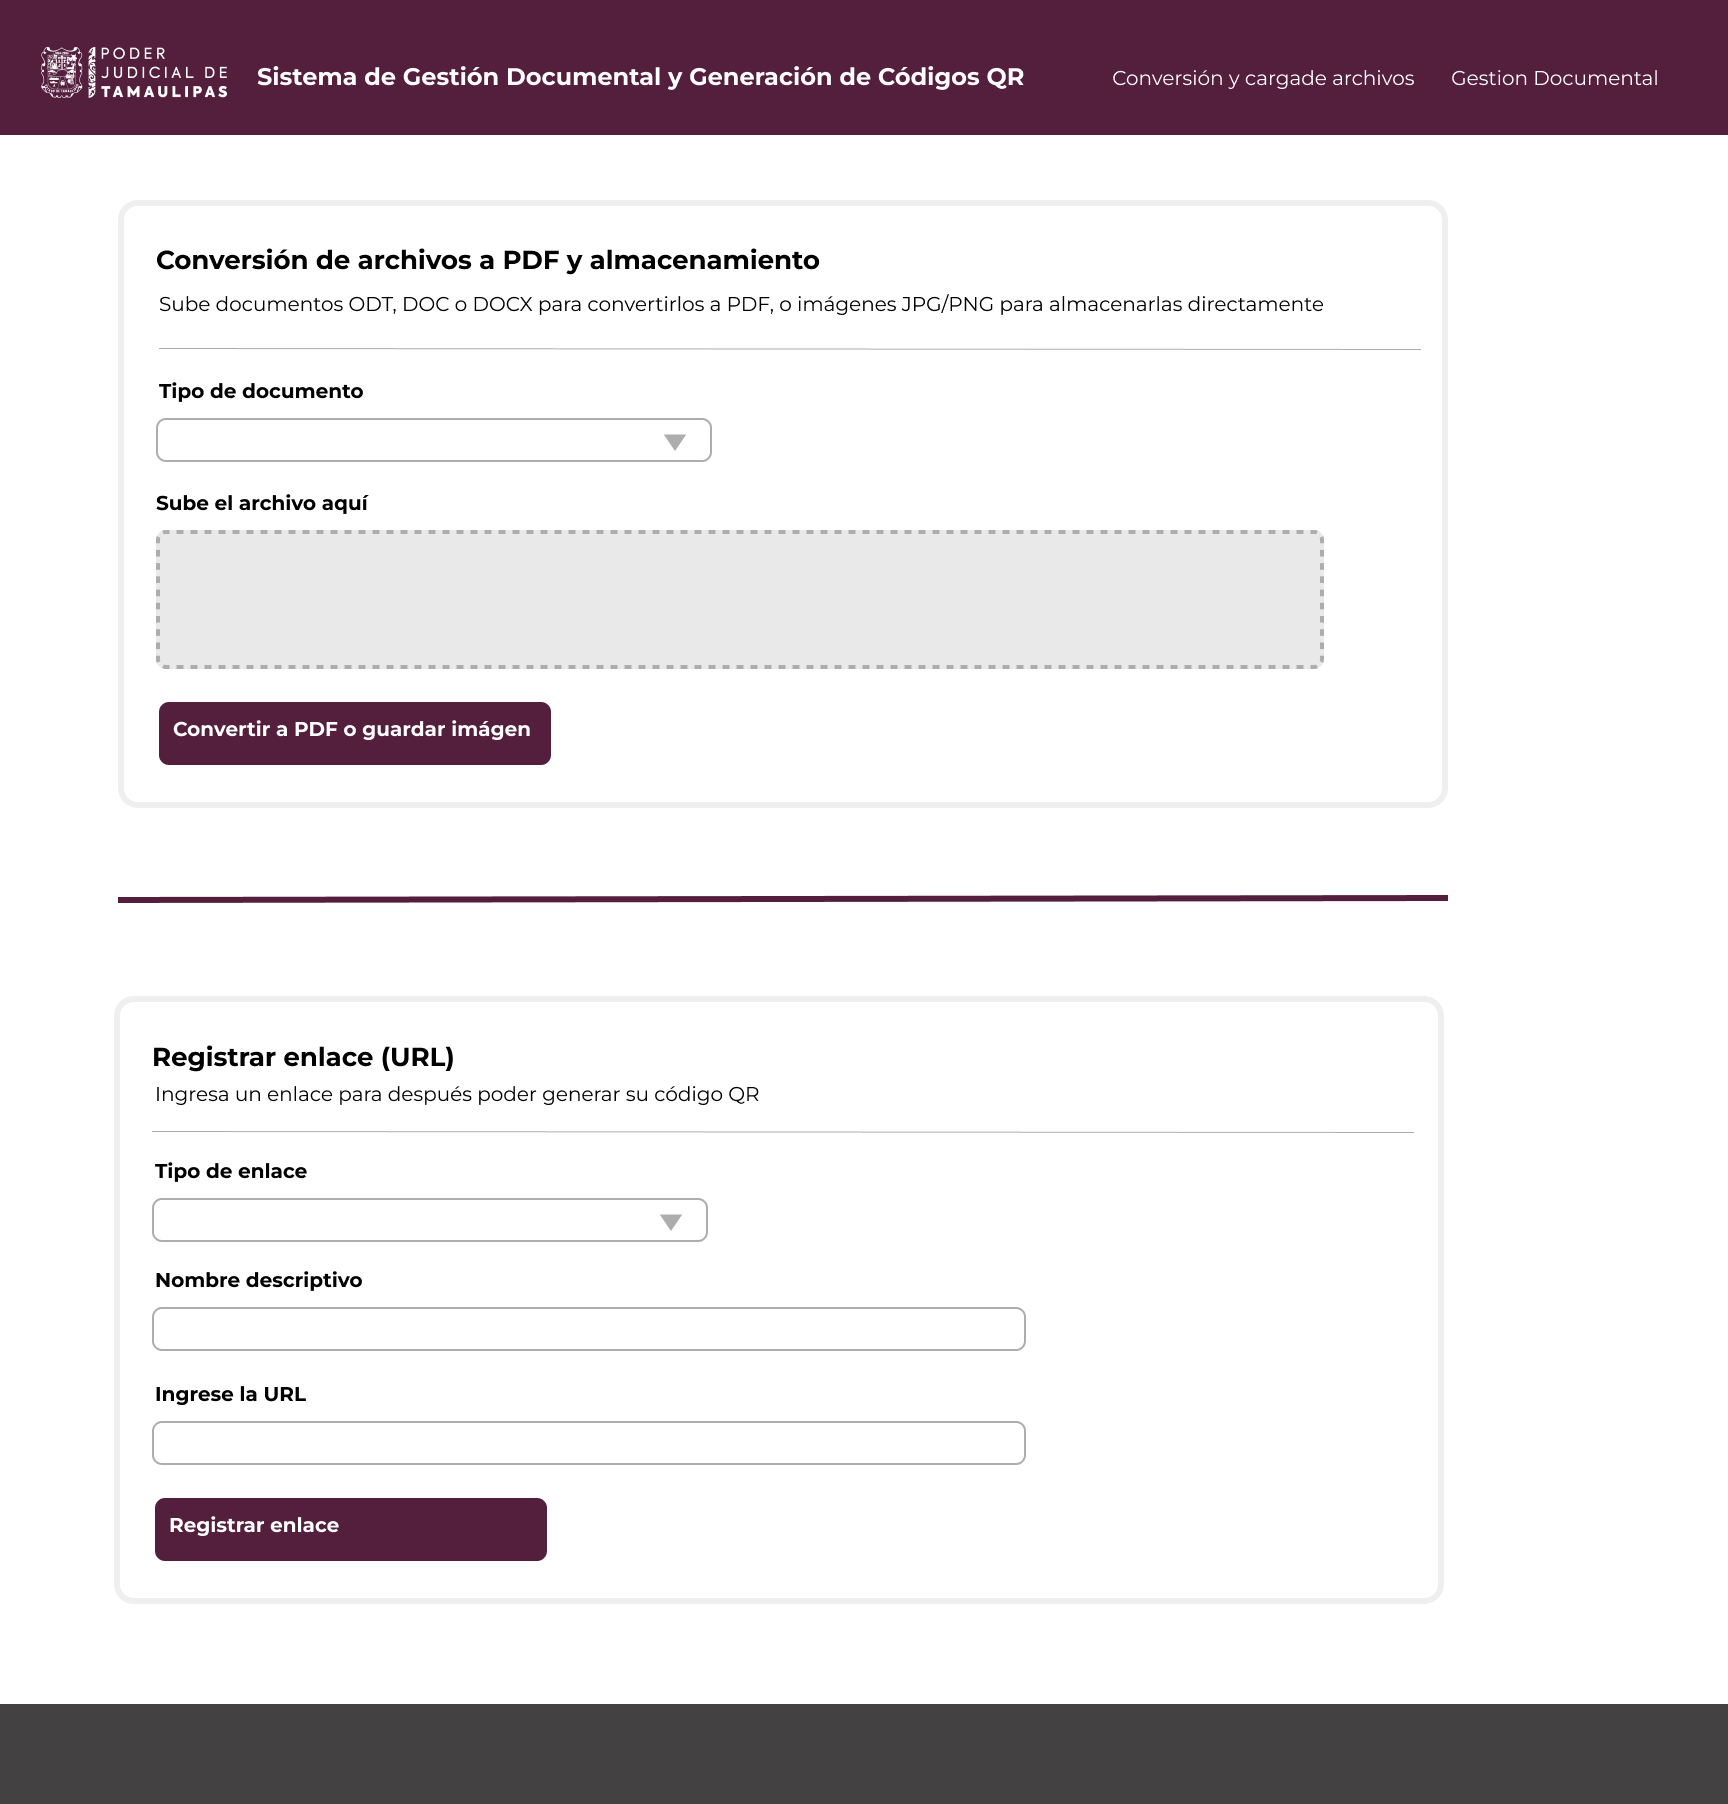
\includegraphics[width=0.7\linewidth]{img/Mockup-Modulo de conversion y carga de archivos.png}
    \caption{Prototipo de la interfaz del módulo de conversion y carga de archivos. Fuente: elaboración propia}
    \label{fig:mockup-1}
\end{figure}

\paragraph{Modulo de conversion y carga de archivos}
En la Figura \ref{fig:mockup-2}
\begin{figure}[!tbh]
    \centering
    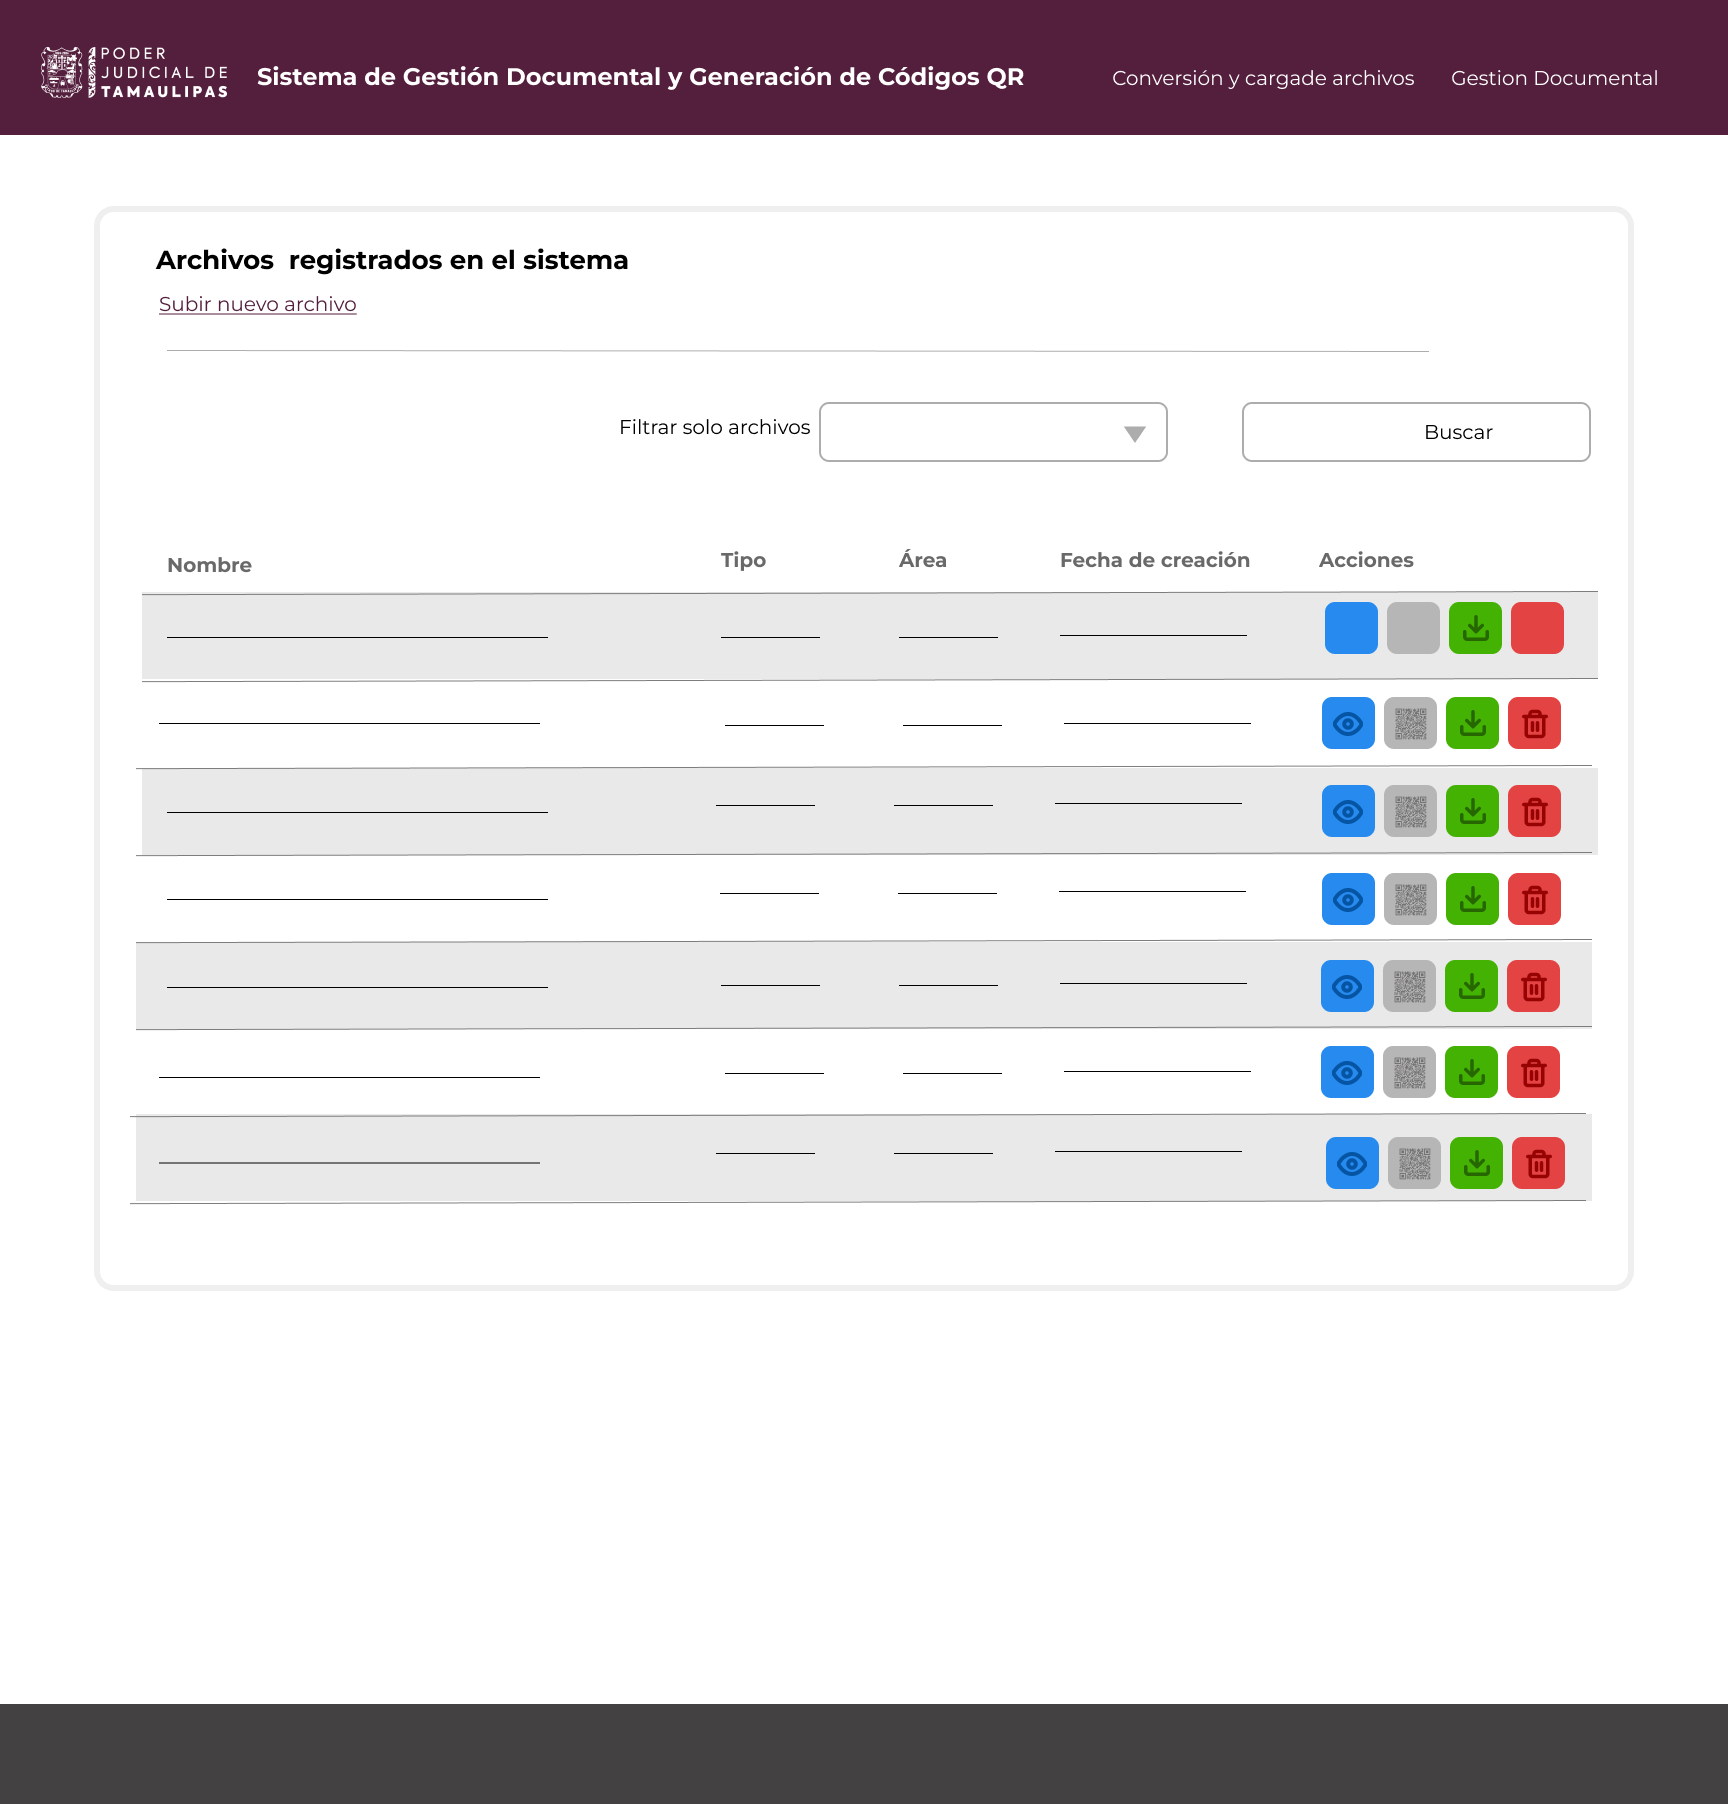
\includegraphics[width=0.7\linewidth]{img/Mockup-Modulo de gestión documental.png}
    \caption{Prototipo de la interfaz del módulo de gestión documental. Fuente: elaboración propia}
    \label{fig:mockup-2}
\end{figure}

\subsection{Desarrollo del sistema}
herramientas, lenguajes de programación y la arquitectura para construir los módulos